\documentclass[a4paper,10pt]{article}
\usepackage{fullpage}
\usepackage[british]{babel}
\usepackage[T1]{fontenc}
\usepackage{amsmath}
\usepackage{amssymb}
\usepackage[T1]{fontenc}
\usepackage{natbib}
\usepackage[utf8]{inputenc}
%\usepackage{amsthm} \newtheorem{theorem}{Theorem}
\usepackage{color}
\usepackage{float}
\usepackage{authblk}
\usepackage{caption}
\DeclareCaptionFont{white}{\color{white}}
\DeclareCaptionFormat{listing}{\colorbox{gray}{\parbox{\textwidth}{#1#2#3}}}
\captionsetup[lstlisting]{format=listing,labelfont=white,textfont=white}

\usepackage{alltt}
\usepackage{listings}
\usepackage{aeguill}
\usepackage{dsfont}
%\usepackage{algorithm}
%\usepackage{algorithmicx}
\lstset{% parameters for all code listings
language=Python,
frame=single,
basicstyle=\small, % nothing smaller than \footnotesize, please
tabsize=2,
numbers=left,
% framexleftmargin=2em, % extend frame to include line numbers
%xrightmargin=2em, % extra space to fit 79 characters
breaklines=true,
breakatwhitespace=true,
prebreak={/},
captionpos=b,
columns=fullflexible,
escapeinside={\#*}{\^^M}
}


% Alter some LaTeX defaults for better treatment of figures:
    % See p.105 of "TeX Unbound" for suggested values.
    % See pp. 199-200 of Lamport's "LaTeX" book for details.
    % General parameters, for ALL pages:
    \renewcommand{\topfraction}{0.9}        % max fraction of floats at top
    \renewcommand{\bottomfraction}{0.8}        % max fraction of floats at bottom
    % Parameters for TEXT pages (not float pages):
    \setcounter{topnumber}{2}
    \setcounter{bottomnumber}{2}
    \setcounter{totalnumber}{4} % 2 may work better
    \setcounter{dbltopnumber}{2} % for 2-column pages
    \renewcommand{\dbltopfraction}{0.9}        % fit big float above 2-col. text
    \renewcommand{\textfraction}{0.07}        % allow minimal text w. figs
    % Parameters for FLOAT pages (not text pages):
    \renewcommand{\floatpagefraction}{0.7}        % require fuller float pages
% N.B.: floatpagefraction MUST be less than topfraction !!
    \renewcommand{\dblfloatpagefraction}{0.7}        % require fuller float pages

% remember to use [htp] or [htpb] for placement


\usepackage{fancyvrb}
%\DefineVerbatimEnvironment{code}{Verbatim}{fontsize=\small
%\DefineVerbatimEnvironment{example}{Verbatim}{fontsize=\small}

\usepackage{url}
\urldef{\mailsa}\path|josh0151@student.uu.se |
\urldef{\mailsb}\path|bjfo5755@student.uu.se |
\urldef{\mailsc}\path|svlu5735@student.uu.se |
\urldef{\mailsd}\path|krjo7211@student.uu.se |
\newcommand{\keywords}[1]{\par\addvspace\baselineskip
\noindent\keywordname\enspace\ignorespaces#1}


\usepackage{tikz} \usetikzlibrary{trees}
\usepackage{hyperref} % should always be the last package

% useful colours (use sparingly!):
\newcommand{\blue}[1]{{\color{blue}#1}}
\newcommand{\green}[1]{{\color{green}#1}}
\newcommand{\red}[1]{{\color{red}#1}}

% useful wrappers for algorithmic/Python notation:
\newcommand{\length}[1]{\text{len}(#1)}
\newcommand{\twodots}{\mathinner{\ldotp\ldotp}} % taken from clrscode3e.sty
\newcommand{\Oh}[1]{\mathcal{O}\left(#1\right)}

% useful (wrappers for) math symbols:
\newcommand{\Cardinality}[1]{\left\lvert#1\right\rvert}
%\newcommand{\Cardinality}[1]{\##1}
\newcommand{\Ceiling}[1]{\left\lceil#1\right\rceil}
\newcommand{\Floor}[1]{\left\lfloor#1\right\rfloor}
\newcommand{\Iff}{\Leftrightarrow}
\newcommand{\Implies}{\Rightarrow}
\newcommand{\Intersect}{\cap}
\newcommand{\Sequence}[1]{\left[#1\right]}
\newcommand{\Set}[1]{\left\{#1\right\}}
\newcommand{\SetComp}[2]{\Set{#1\SuchThat#2}}
\newcommand{\SuchThat}{\mid}
\newcommand{\Tuple}[1]{\langle#1\rangle}
\newcommand{\Union}{\cup}
\usetikzlibrary{positioning,shapes,shadows,arrows}
% SRS commands
\newcommand{\requirement}[1]{\subsubsection{#1}\begin{tabular}{l p{12.2cm}}}

\newcommand{\reqsection}[1]{\\ \textbf{#1} &}

\newcommand{\stoprequirement}{\end{tabular}}

\newcommand{\prio}[2]{\texttt{Priority:} #1 \emph{Motivation:} #2}

\usepackage{url}



\title{\textbf{DragonQuest report, group 10}}

\author{Bj{\"o}rn Forsberg, Jonathan Sharyari, Sven Lundgren, Kristian Johansson}
\textwidth 5.5in
\oddsidemargin 0.5in


\begin{document}

\maketitle

% DICTIONARY
% ----------
% The project: �vergripande om hela projektet, inkl. br�dspel, kod, diagram, etc.
% The game: Abstrakt om spelets funktionalitet i systemet, samt konkret om br�dspelet.
% The system: Konkret om v�r modellering av spelet.
% Subsystem: The packages
% Packages: The packages, when we look at them from a lower level.
% NOTE: At points, the words may be used interchangably.

\section{Introduction}

The goal of this project is to design and implement a computer game adaptation of the \emph{DragonQuest} board game. A subgoal of the project is making the game architecture losely coupled with the actual game, to allow the reuse of the architecture and its components to implement other similar games. 

\subsection{The DragonQuest board game}

The \emph{DragonQuest} game is a turn-based board game for one or more players. The main goal of the game is to enter an old castle and finding the way to the treasure chamber, rumored to be full of unclaimed treasure. The castle consists of a number of rooms which are guarded by monsters and traps, and the treasure chamber itself is guarded by a sleeping dragon.

The players have to find their way through the castle, collect as much treasure as possible, and not get killed by monsters before the end of the day, as no human can survive the night in the castle.

The rooms are connected through doors, both regular and hidden, limiting the possible moves through the castle, thereby forcing the player to always keep the time needed for escaping the castle in mind, while working their way into the inner castle in search of treasure.

All actions by the players result in different reactions from the game, represented by drawing different cards. These cards are divided into different stacks depending on their functionality. There is, for example, a Room Search Card stack deciding the outcome of a room search, and a Door Card stack for deciding if a locked door is opened or remains closed.

The game is over when the day has passed, and the player that has managed to collect the largest treasure and escape the castle alive is pronounced the winner.

\subsection{The computer game adaption}

The computer game adaption is built around a set of modules with independent functionality needed to play the game, these include a module for representing the game board, and a module for performing battles. The game rules are implemented using an object representing the cards in the board game. This implementation allows for simple changes to the game rules, should we want to change them in future updates, while it keeps the game structure closely linked to that of the board game, ensuring that the game behaves in a way similar to the board game, as this is one of the non-functional requirements for the game. Section \ref{classdiagram} contains a more in-depth presentation of the internal structure of the computer game.

\subsection{Artifacts}

The design process produces a number of artifacts used to describe the system under design. A more comprehensive documentation of these artifacts follow later in this report, but they are presented in short here to give the reader an overview of the concepts used and how they relate to each other. The major artifacts of the project are:

\begin{itemize}
\item Analysis artifacts
  \begin{itemize}
    \item Software Requirement Specification
    \item Use Cases
    \item Domain Model
  \end{itemize}
\item Design artifacts
  \begin{itemize}
  \item Class diagrams
  \item System architecture diagram
  \item Dynamic diagrams
  \end{itemize}
\end{itemize}

The \emph{Software Requirement Specification (SRS)} contains all the requirements, both \emph{functional} and \emph{non-functional}. These requirements dictate what the system shall do, and how it shall do it. The SRS is presented in Section \ref{sec:srs}.

The \emph{Use Cases} are produced during the analysis of the board game to express the functionality of the system from different users viewpoint. The use cases are presented in Section \ref{sec:usecases}.

Both the SRS and the Use case artifacts are a great help both in the design of the system, and to verify that the system actually performs as specified, as it outlines the inner functionality of the system, and the interactions with different users respectively. With the help of these two artifacts a \emph{Domain Model} can be produced, describing the objects that make up the game and their relations. This document in turn is used to get a graspable overview of the game the system will module and will be a great reference when designing the actual system. The Domain Model is presented and discussed in more detail in Section \ref{sec:domainmodel}.

The produced analysis artifacts are, as previously pointed out, used as the foundation to construct the design artifacts. The Domain Model can be used to construct the first basic \emph{Class Diagram}, as the concepts and relations described by the domain model must be implemented by the system anyway. The iterative process of deciding which concepts from the domain model should be turned into classes, which should be represented otherwise, and how to implement their relations produces a implementable class diagram from the domain model. A more thourough presentation of the class diagram for this system is available in Section \ref{sec:staticdiagrams}.

As the design of the system gets more and more clear from the Class Diagram, it is possible to start dividing the functionality into clearly divided subsystems or modules. At this point another level of abstraction can be introduced, by creating a \emph{System Architecture Diagram}, only describing the subsystems and their interactions. If the designer is more experienced the system architecture diagram could be designed before the class diagram, to ensure that the system conforms to a pre-defined divison of focus areas, but in this project the class diagram was iteratively improved until an architecture emerges. Further information about the System Architecture Diagram can be found in Section \ref{sec:architecture}.

The \emph{Dynamic diagrams} are a way of presenting the interactions done in the system to fulfill a predefined requirement or use-case, to demonstrate how a specific problem has been solved. These diagrams can also be used to verify that the system is actually able to perform the intended actions, without breaking important object oriented design concepts as low coupling and information hiding. The dynamic diagrams produced during this project are presented in Section \ref{sec:dynamics}.

\subsection{Methodology}

The game design is done in an iterative fashion, working on multiple parts of the design at once, refining them as the project continues. This approach grants the designer the possibility to convert the domain model part by part to a class diagram, focusing on areas given the highest priority first, using Design Patterns on a well defined scope of the system. Once the first version of the class diagram is finished, the class diagram can be iteratively improved by using concepts such as Anti-Patterns and the GRASP method to identify weaknesses and adjust the design to overcome them.

The iterative approach also grants us the possibility to start coding at an earlier stage, which can also help identify weaknesses and bad design decisions. It also produces runnable code at an earlier stage in the project process, which can be used to convince external stakeholders, like the customer, that progress is being made. This will also allow this stakeholder to give early input on the design to continously ensure that the correct product is produced.


\section{Domain Model}
\label{sec:domainmodel}

\begin{figure}[h]
\center
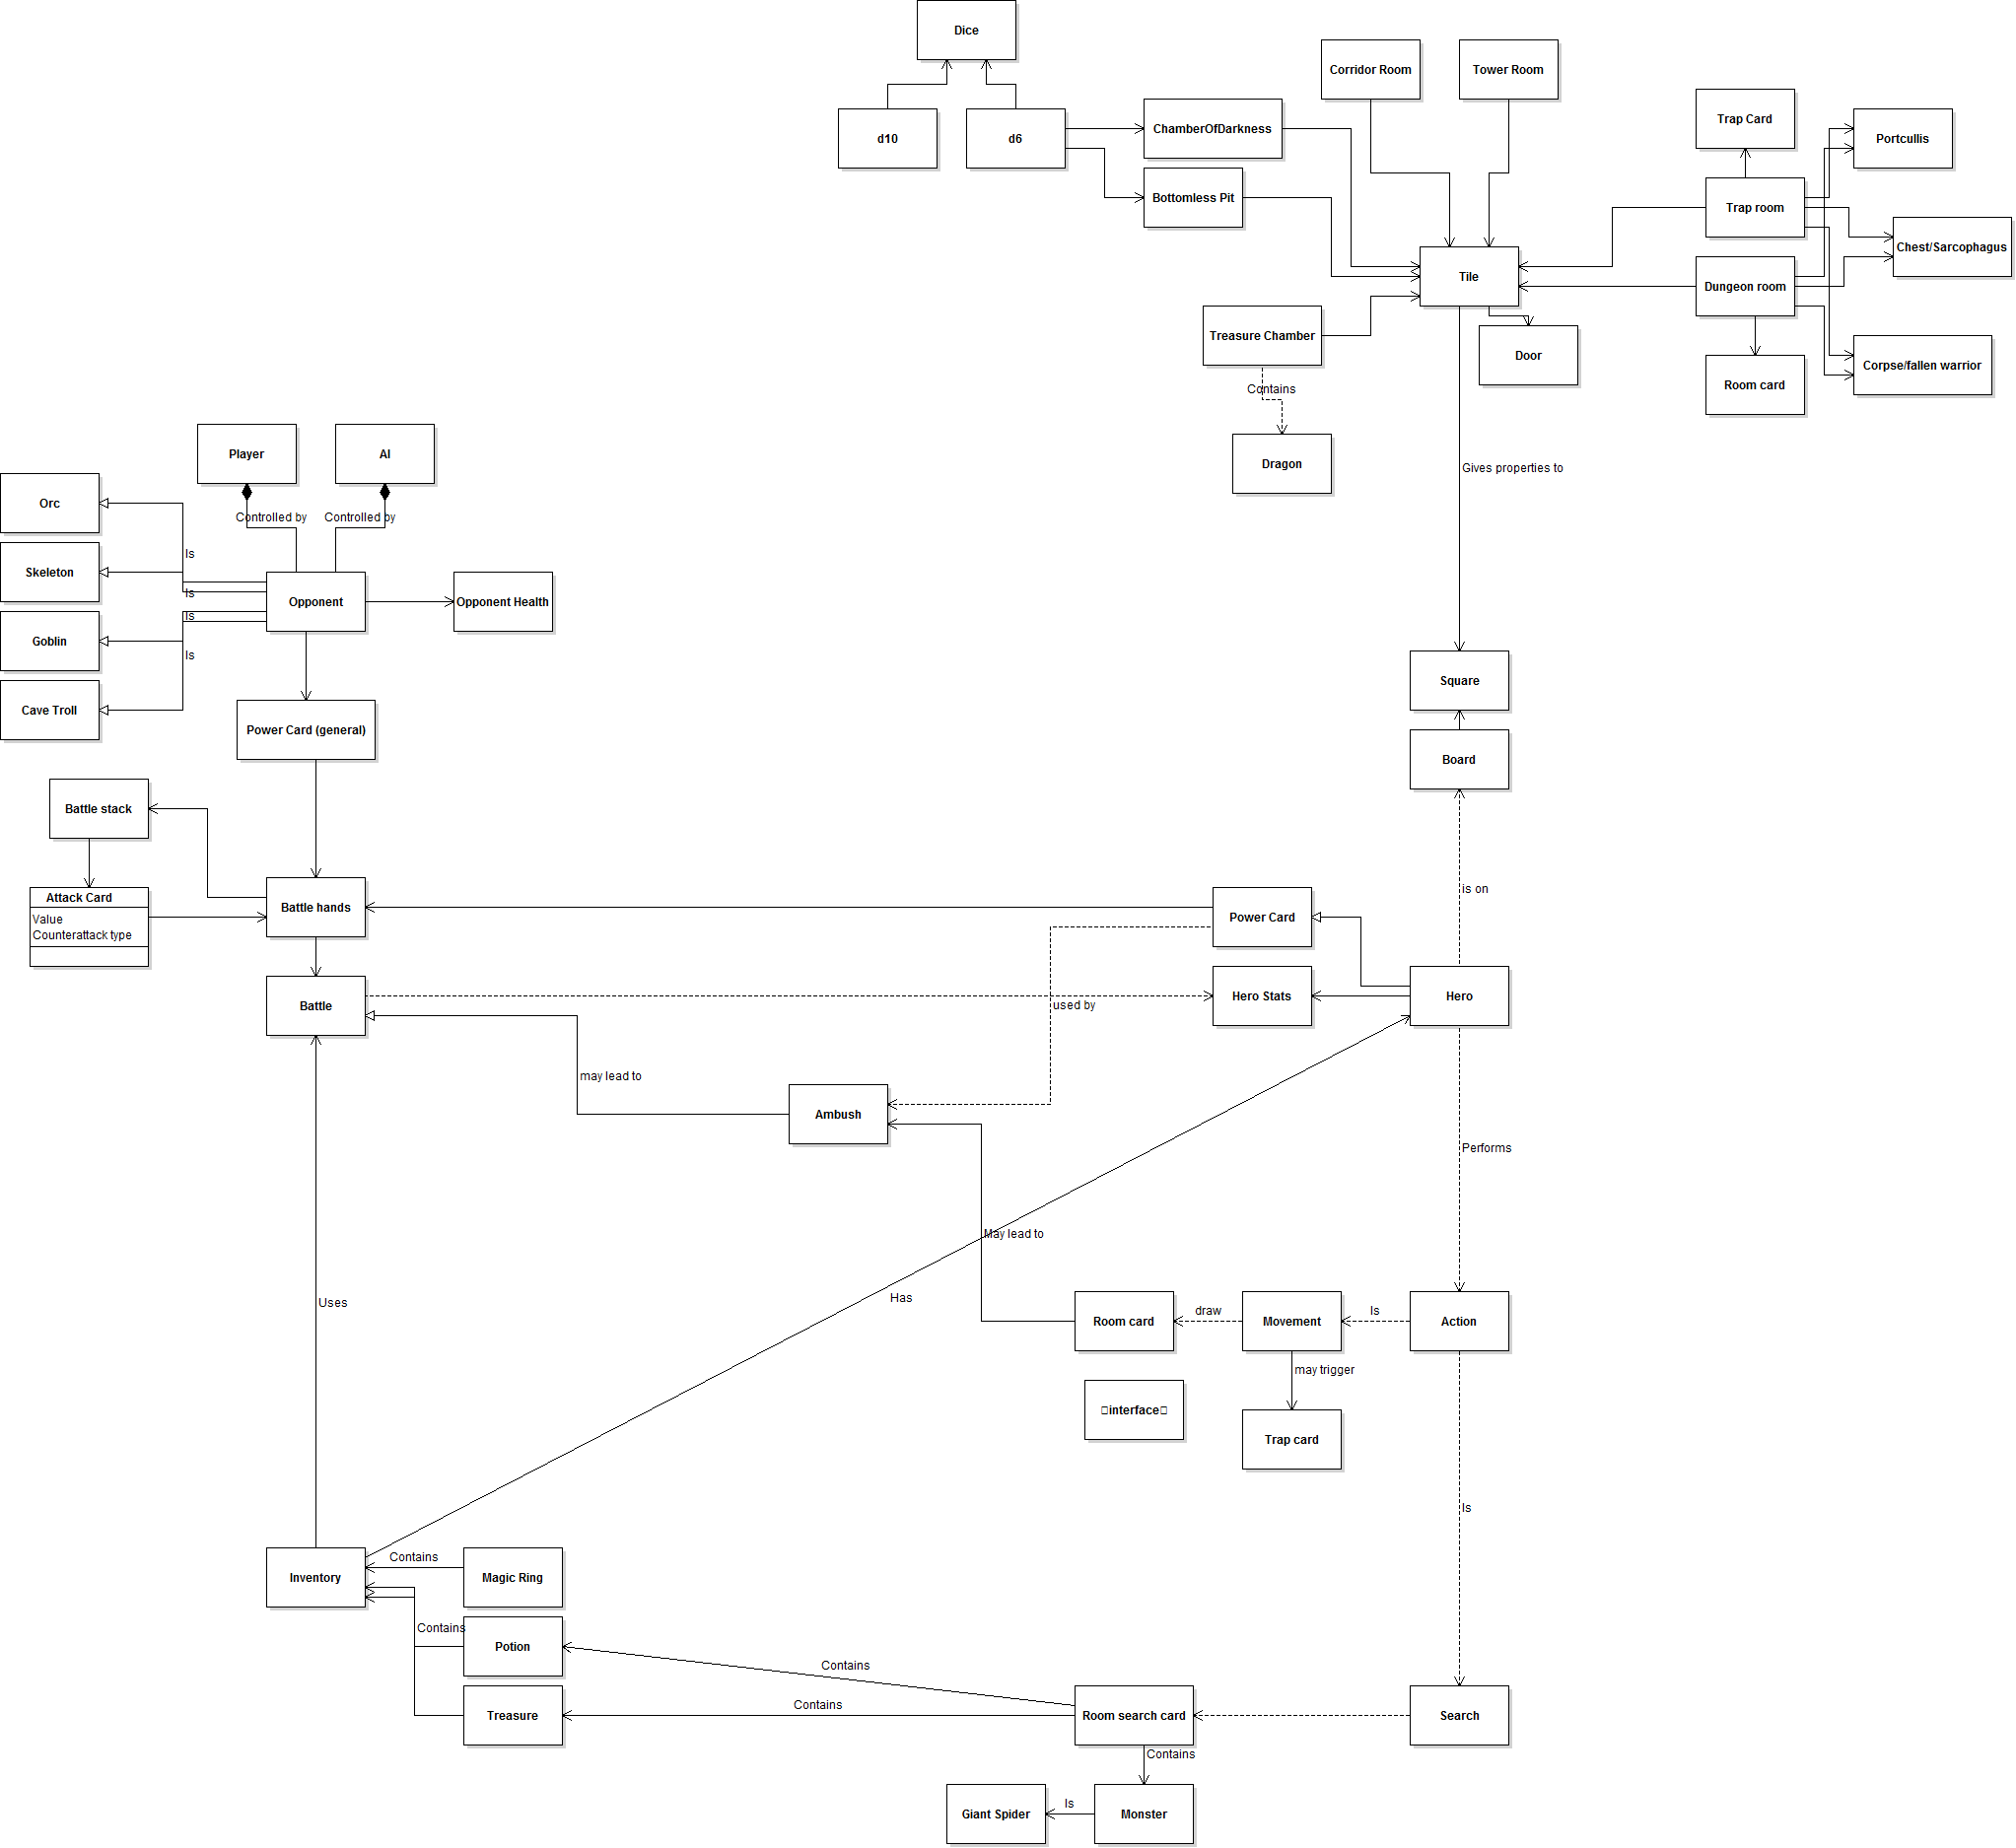
\includegraphics{diagrams/DomainModel.png}
\caption{The domain model for the game. The arrows may be misleading as the relation sometimes goes in both directions, so use caution when interpreting them.}
\label{fig:domain_model}
\end{figure}

The Domain Model is an analysis artifacts that helps the designer create an understanding of the objects and concepts used in the game the software will model. It visualizes how objects relate to each other and gives the designer a better understanding of the elements of the game. By reading through the game rules and description we can extract a set of nouns used within the game, and place them as objects in our model, together with the interactions between the objects. This is a great help when deciding which objects belong together and may make up a subsystem in the software implementation. The domain model for the DragonQuest game is displayed in Figure \ref{fig:domain_model}.

From the domain model it is immediately clear that the game board (\textsc{Board}) and the objects associated with it is a clear candidate for a subsystem, as is the battling part of the game. This modularity is transferred to the class diagram, presented in Section \ref{classdiagram}.




\section{Design - Static Diagrams}
\label{sec:staticdiagrams}

\begin{figure}[]
\center
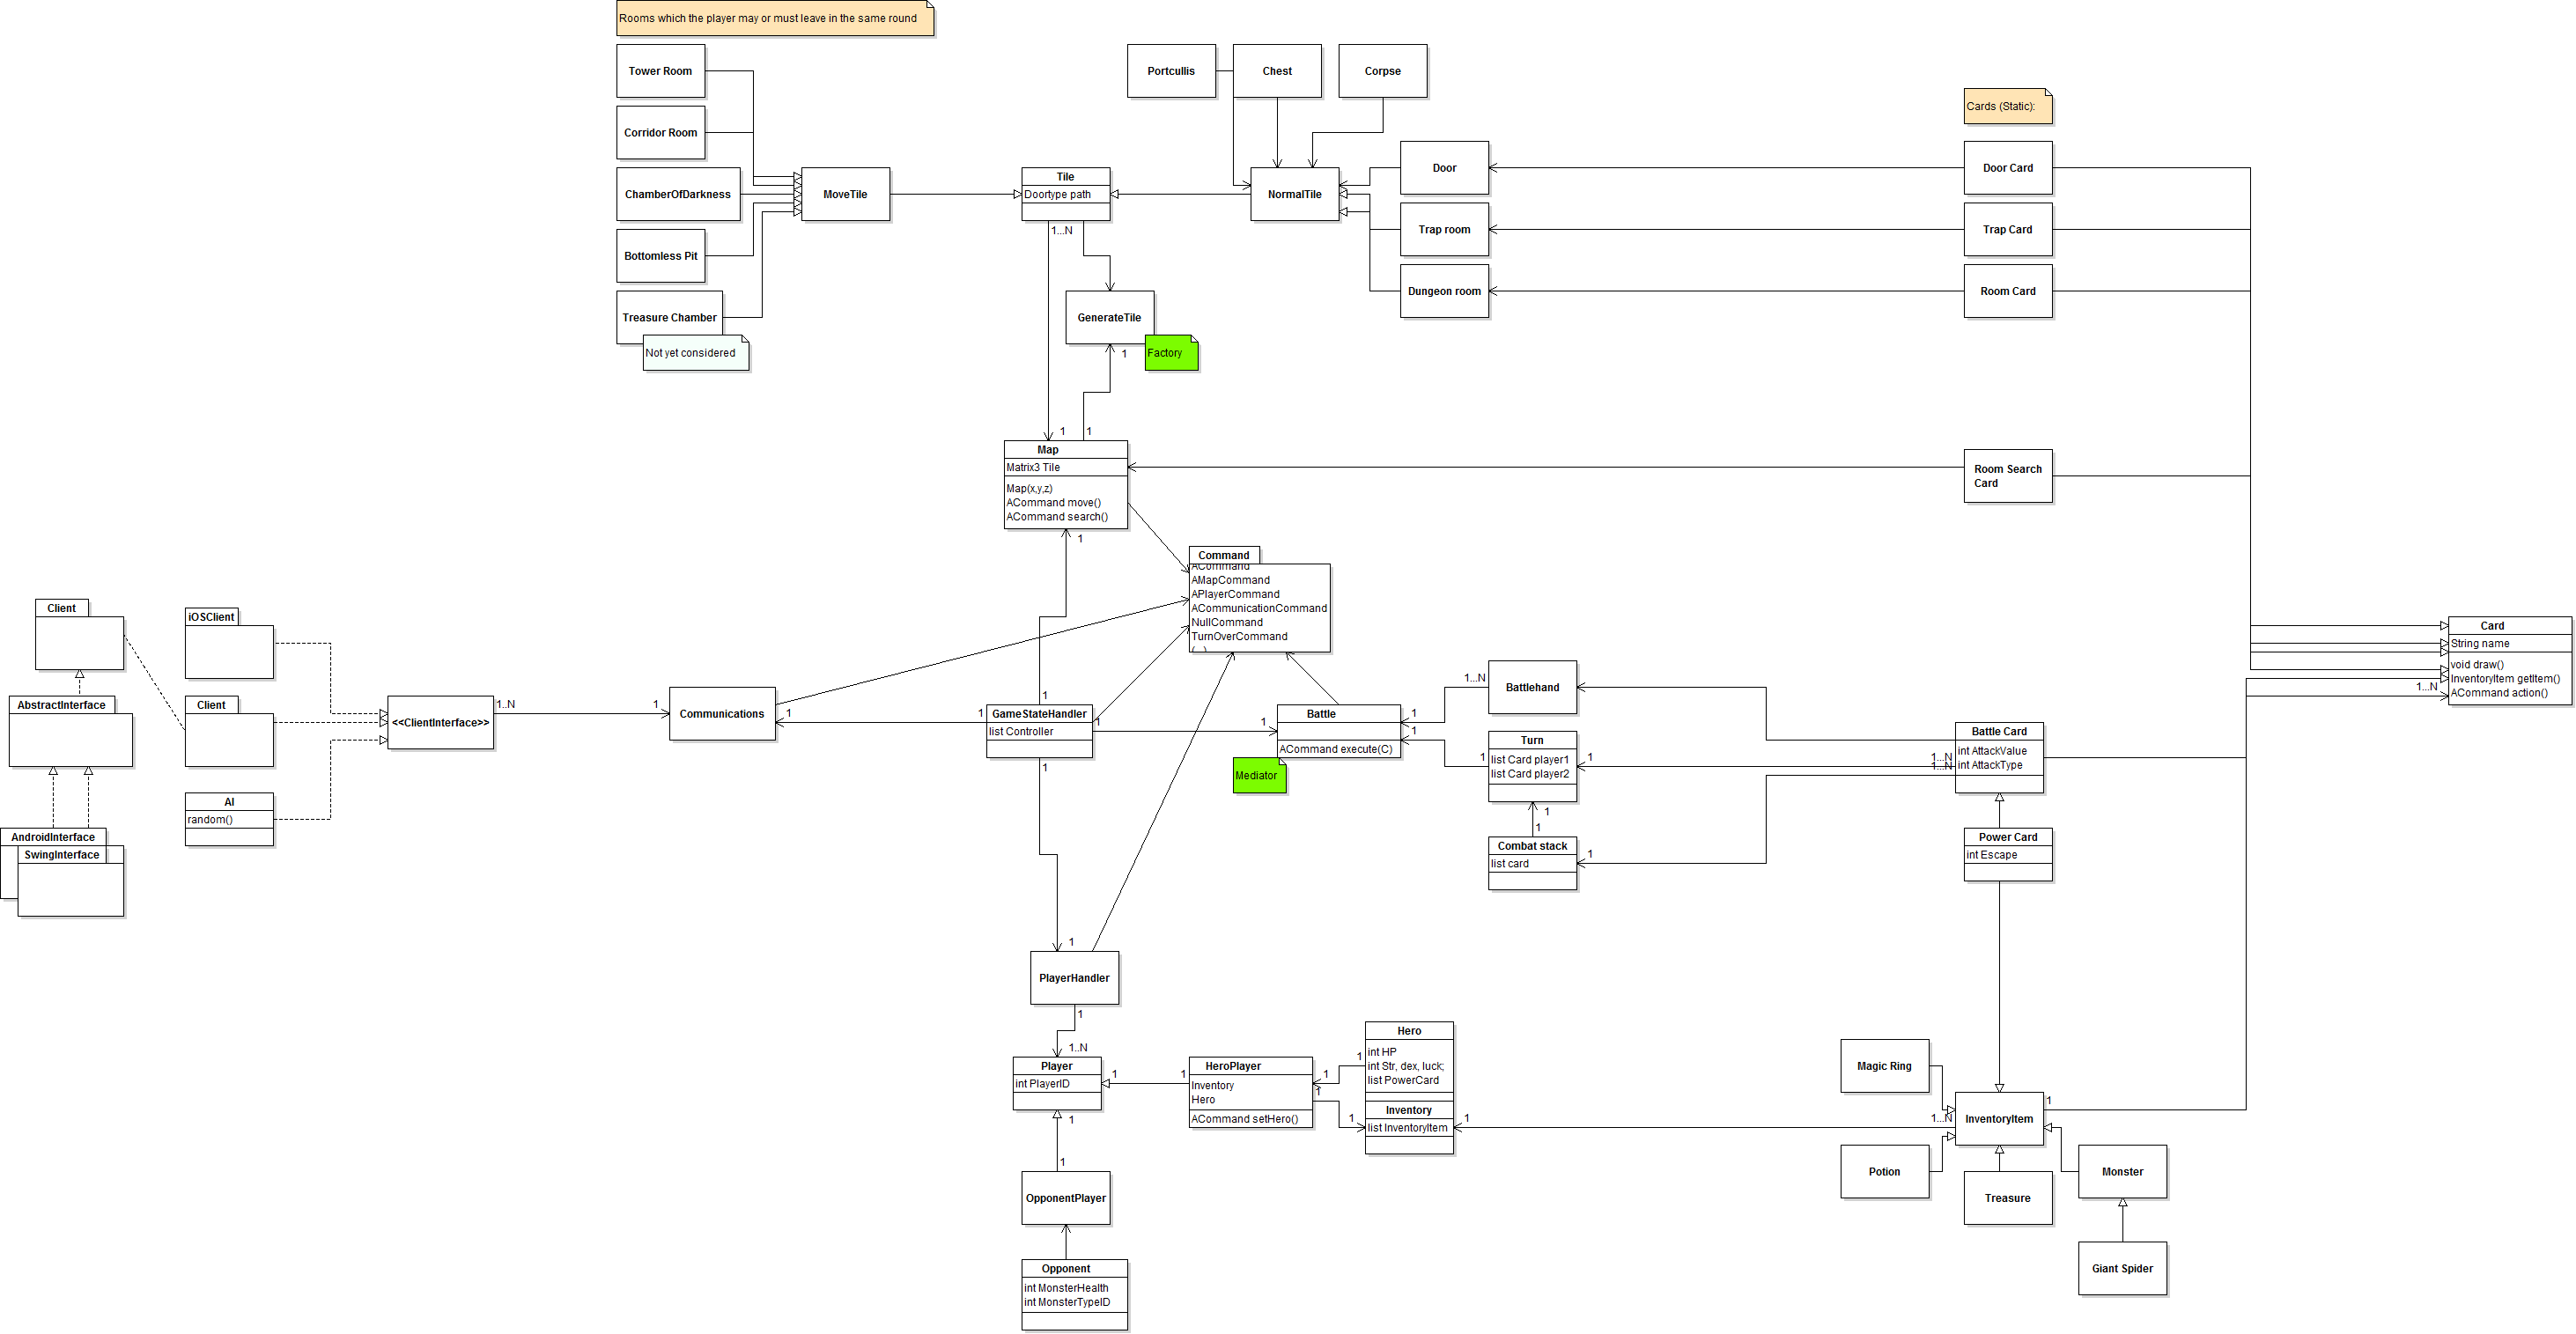
\includegraphics[width=1.65\textwidth,angle=90] {diagrams/ClassDiagram.png}
\caption{The produced class diagram.}
\label{classdiagram}
\end{figure}


\begin{figure}[]
\center
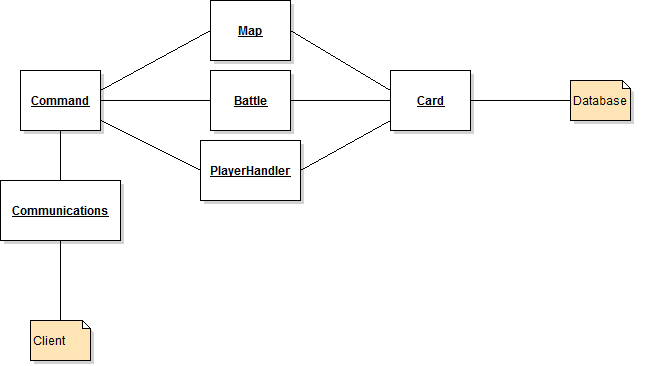
\includegraphics[width=0.9\textwidth] {diagrams/ArchitectureDiagram.png}
\caption{Architecture diagram of the project.}
\label{architecture}
\end{figure}


The game is designed to be a multi-platform, multi-player game, available to a multitude of platforms. In order to achieve this, the game is written in the JAVA programming language, which is supported by all major platforms available today, with the exception of the iOS. To make the game available to also to the iOS, an additional client need be written in Objective-C. By moving most game logic to the server side, the cost and effort required to design the clients is reduced. Clients are only responsible for the graphical representation of the game, and may represent the gamestate in varying ways as long as the communication between the server and the client follows the communication API, which at this point of the design has not yet been decided upon. This also allows for user-generated clients to be designed. In Figure \ref{architecture}, the server-client structure is represented by the line connecting \texttt{client} and \texttt{communications}.

The diagram in Figure \ref{architecture} describes different packages within the game illustrated by white boxes, and additionally communication with external information sources, \texttt{client} and \texttt{database}. All classes seen in Figure \ref{classdiagram} are part of one of the packages in the architecture diagram, see Section \ref{packagestructure} for the exact distribution.


\subsection{Command Package}
The \texttt{command} package is in some sense the heart of the system implementation. All communication between packages (the \texttt{Card} package excluded) goes through the \texttt{command} package as a relay, which keeps the coupling low within the system. The \texttt{GameStateHandler} class has the main responsibility of executing commands, and is able to do so without any knowledge of the nature of the command it executes. As long as there are commands on the command stack, they will be executed until a \texttt{TurnOverCommand} is received, on which point the \texttt{GameStateHandler} sends a query to the player whose turn it is.

When a subsystem needs to send a request or invoke an action in another subsystem, it will generate a command of a type that is destined for the subsystem in question. There are four types of abstract commands, \texttt{MapCommand}, \texttt{CommunicationCommand}, \texttt{PlayerCommand} and \texttt{BattleCommand}, with the destination subsystems as indicated by the names. Each of these command types have concrete commands connected to them, an overview of the (not yet complete) structure of the commands can be see in Figure \ref{commandstructure}.

Note that subsystems do not send commands to the \texttt{GameStateHandler}, but rather respond to calls from the \texttt{GameStateHandler} with new commands, and all commands always respond with a new command with the exception of the \texttt{NullCommand} and the \texttt{TurnOverCommand}. An example of this can be seen in Figure \ref{commandsequence}.

An implication of this structure is that the rules of the game are not highly coupled with the game, instead residing in the ‘’leaves’’, in most cases the Cards. Cards all have a Command connected to them and receiving a card will cause that command to be invoked. Adding new rules to the game will then often be as easy as to add a new type of card to the game. As an example, say a card would be added that allows the player to move an additional time during his/her round, a card that can be found when searching a room. This would be implemented by adding a new card of the type \texttt{SearchCard}, which generates a \texttt{MoveQueryCommand} (does not yet exist), and no other changes to the program would be needed.


\begin{figure}[]
\center
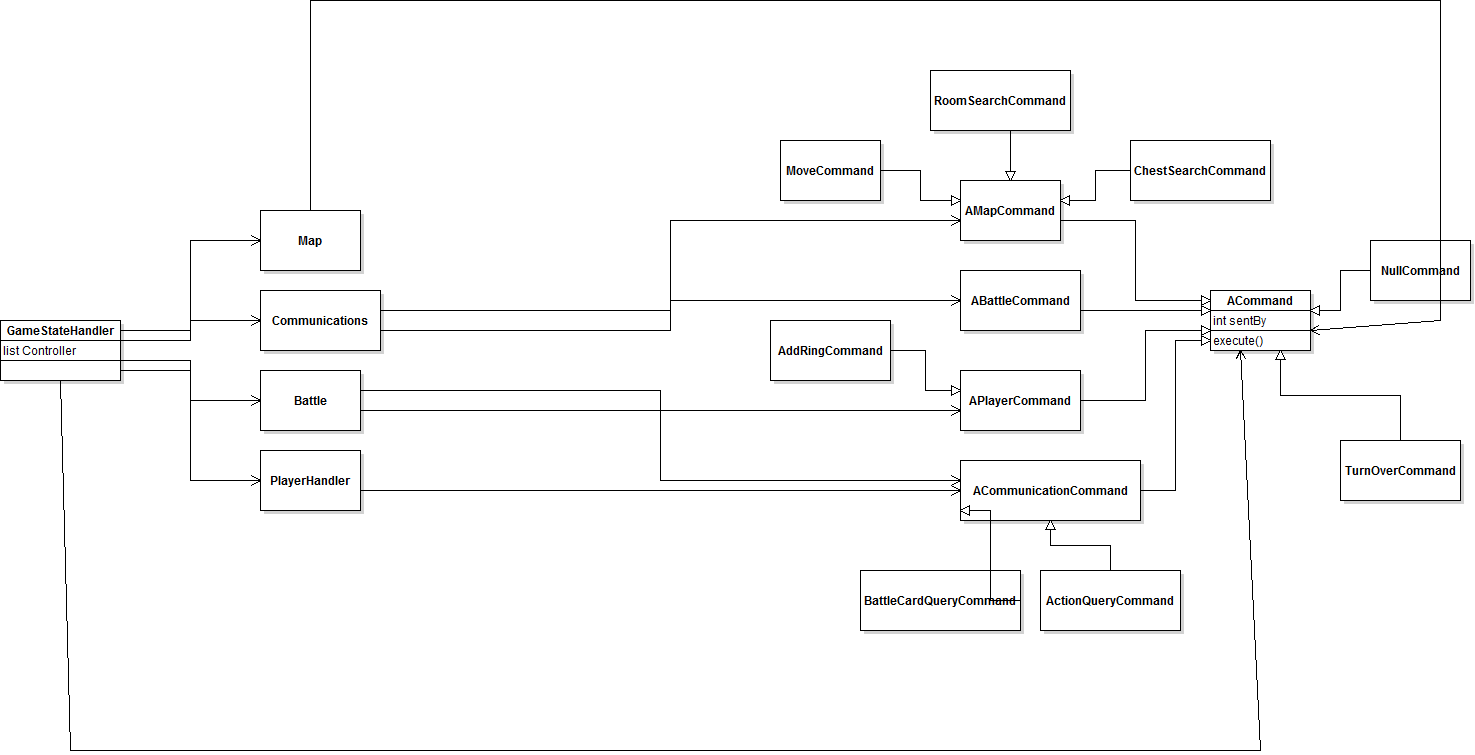
\includegraphics[width=0.9\textwidth] {diagrams/CommandStructureDiagram.png}
\caption{Structure of Commands.}
\label{commandstructure}
\end{figure}

\begin{figure}[]
\center
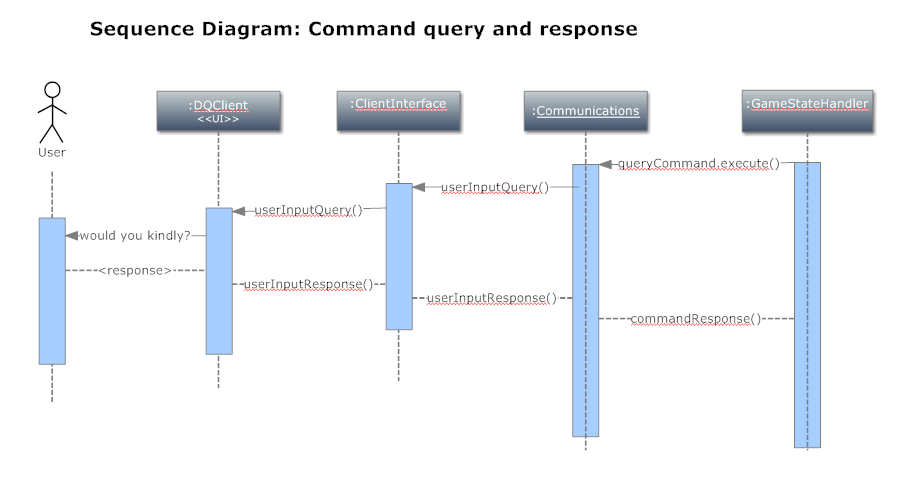
\includegraphics[width=0.9\textwidth] {diagrams/moveCommandSequenceDiagram.png}
\caption{Command query and response.}
\label{commandsequence}
\end{figure}


\subsection{Package Structure}
\label{packagestructure}
\begin{itemize}
\item
Map (package)
	\begin{itemize}
	\item
	Map (class) - Map is responsible for keeping track of the game board, positions of players and includes methods to perform actions on the map, such as \texttt{move}.
	\item
	GenerateTile - GenerateTile is responsible for creating a new random Tile, that makes sense in its current position (doors do not lead into walls for example).
	\item
	Tile - abstract class for tiles, the different concrete subclasses define what kind of tile that is generated by GeneraTetile. Each subclass encapsulates 	 tile specific information.
	\end{itemize}
\item
Battle (package)
	\begin{itemize}
	\item
	Battle (class) - Battle is a mediator (see Mediator design pattern) in the battle sequence and makes sure it calls the correct objects involved in the battle.
	\item
	Battlehand - Each player involved in the battle has a battlehand which holds the battle cards corresponding to that player.
	\item
	Combatstack - Combatstack holds all all of the loser's cards. When a death blow occurs, the cards used to deliver the death blow are removed from the combat stack.
	\item
	Turn - Turn holds the battle cards that have been played by each player during that specifc turn.
	\end{itemize}
\item
PlayerHandler (package)
	\begin{itemize}
	\item
	PlayerHandler (class) - Playerhandler is responsible for managing the players that are involved in the game and stores a list of these.
	\item
	Player - Player is the abstract class for the different kinds of players that exist.
	\item
	HeroPlayer - Represents a player in the game that has a hero associated with itself.
	\item
	OpponentPlayer - Represents opponents of heroes in battles, for example different kinds of monsters.
	\item
	Hero - The hero is what is referred to as the hero in the actual piece that corresponds to the player. Holds an invetory of items.
	\item
	InventoryItem - The inventory of a player holds all different kinds of items a hero can hold, like different types of cards, potions and other artefacts.
	\end{itemize}
\item
Communications (package)
	\begin{itemize}
	\item
	Communications (class) - Communications is responsible for communicating with the ClientInterface and send the correct commands.  
	\item
	ClientInterface - An interface for how to talk to the multiple different clients that exists (clients could be AI or different implementations of a UI).
	\item
	AI - In any scenario where a user client can't respond to a query, AI is used and will generate a response according to the AI implemenation.
	\item
	Client - Is the actual user client which the user communicates with.
	\end{itemize}
\item
Command (package)
	\begin{itemize}
	\item
	ACommand - Abstract command which all command types inherit from. Commands are an essential part of the system and are used to be able to perform actions, all executed in gamestatehandler.   
	\item
	GameStateHandler - The gamestatehandler has several responsibilities. It holds an instance of the map, playerhandler and communications class. This is also where all commands are executed. Furthermore it keeps track of which player's turn it is and how many turns there are left in the game. 
	\end{itemize}
\item
Card (package)
	\begin{itemize}
	\item
	Card (class) - Abstract card class which all different cards in the game inherit from. Cards are used in several different subsystems and their implemantation vary quite a bit as a card can be anything from a battle card used in a battle, a room search card containing an item to a room card specifying an ambush.   
	\end{itemize}
\end{itemize}


\section{Dynamic Diagrams}
\label{sec:dynamics}
Battle Module
\begin{figure}[h]
\center
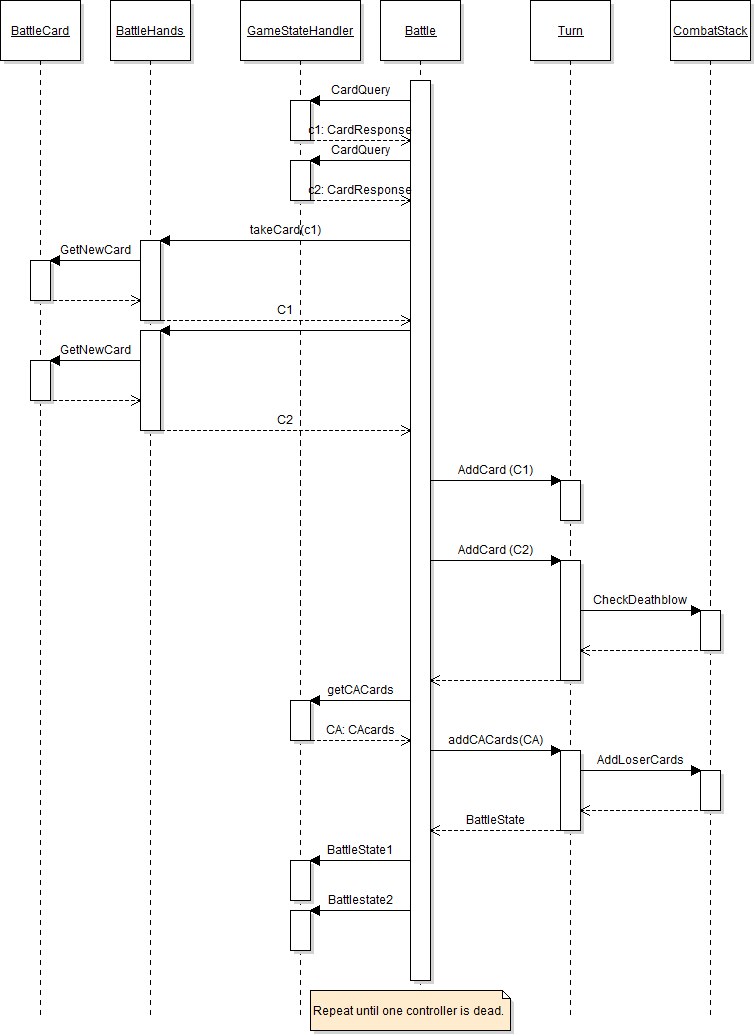
\includegraphics{diagrams/BattleSequenceDiagram.png}
\caption{A sequence diagram of one turn for each participant in a battle.}
\label{fig:battle_sequence_diagram}
\end{figure}

\begin{figure}[h]
\center
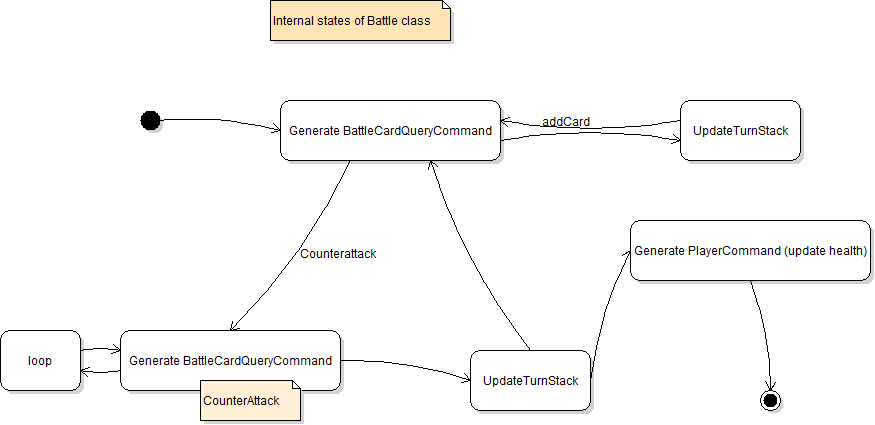
\includegraphics{diagrams/BattleStateDiagram.png}
\caption{A state diagram explaining the internal states of the Battle class.}
\label{fig:battle_state_diagram}
\end{figure}


A battle is conducted between two heroes controlled either by human players or by the AI. For more information on how a battle is conducted, see use case \ref{fightopponent}.

Diagram \ref{fig:battle_sequence_diagram} models one turn out of many in a battle. The \emph{GameStateHandler} communicates with human players and the AI through means not shown in this diagram, and the response is in the form of a card in the respective participant's battle hand. The class \emph{Battle} acts as a mediator between the heroes, their battle hands and \emph{turn}. A battle hand is composed of the five cards currently available to the respective player. The turn class contains the logic determining the winner of a single battle turn by comparing the chosen cards and possible lingering effects from previous rounds (specifically \emph{death blows}, see use case \ref{fight_deathblow}). When a turn ends, the losers' cards are added to the combat stack.

Diagram \ref{fig:battle_state_diagram} models the behaviour of the battle class from the start until the end of a battle.

\begin{figure}[h]
\center
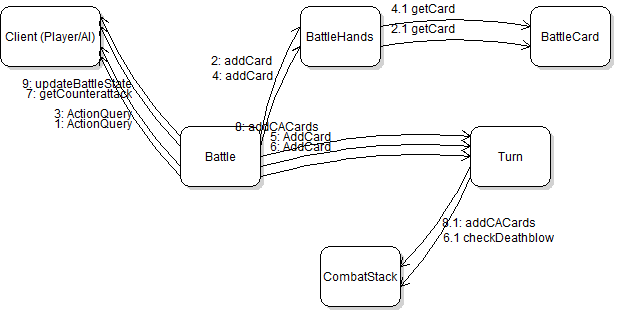
\includegraphics{diagrams/CounterAttackCommDiagram.png}
\caption{A diagram explaining the communication between the participating classes when a counter attack is possible.}
\label{fig:counter_attack_comm_diagram}
\end{figure}

A counter attack is possible in each turn for the losing participant given certain circumstances. For more detail on counter attack see use case \ref{fight_counterattack}. Diagram \ref{fig:counter_attack_comm_diagram} models the communication between the classes participating in a single turn when a counter attack is possible.


\begin{figure}[h]
\center
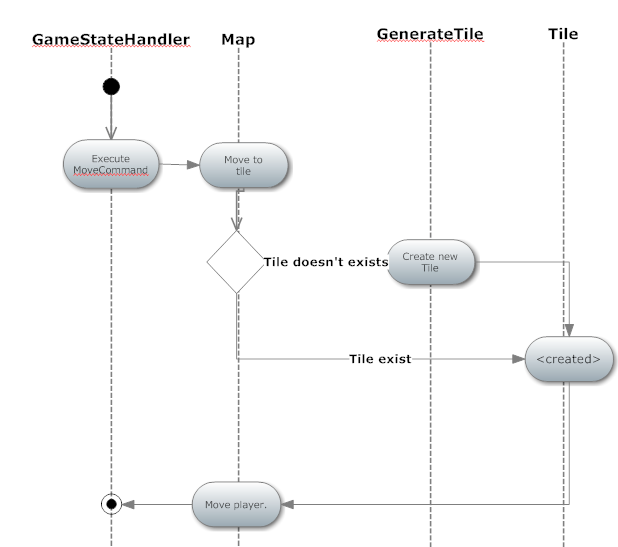
\includegraphics{diagrams/moveActivityDiagram.png}
\caption{An activity diagram explaining the process of a hero moving to a new square and the possible creation of a new tile.}
\label{fig:move_activity_diagram}
\end{figure}

Diagram \ref{fig:move_activity_diagram} models the process of a hero moving to a new room. For further information on how a move is carried out, see use case \ref{moveoutofroom}. A \emph{tile} is created if the room has previously not been visited, otherwise the hero simply moves to the new room.





% Place all outstanding floats
\clearpage

\section*{Appendices}

\appendix

\documentclass[a4paper,10pt]{article}
\usepackage{fullpage}
\usepackage[british]{babel}
\usepackage[T1]{fontenc}
\usepackage{amsmath}
\usepackage{amssymb}
\usepackage[T1]{fontenc}
\usepackage[latin1]{inputenc} 
%\usepackage{amsthm} \newtheorem{theorem}{Theorem}
\usepackage{color}
\usepackage{float}



\usepackage{caption}
\DeclareCaptionFont{white}{\color{white}}
\DeclareCaptionFormat{listing}{\colorbox{gray}{\parbox{\textwidth}{#1#2#3}}}
%\captionsetup[lstlisting]{format=listing,labelfont=white,textfont=white}


\usepackage{alltt}
\usepackage{listings}
 \usepackage{aeguill} 
\usepackage{dsfont}
%\usepackage{algorithm}
%\usepackage{algorithmicx}
\usepackage{subfig}
\lstset{% parameters for all code listings
	language=Python,
	frame=single,
	basicstyle=\small,  % nothing smaller than \footnotesize, please
	tabsize=2,
	numbers=left,
%	framexleftmargin=2em,  % extend frame to include line numbers
	%xrightmargin=2em,  % extra space to fit 79 characters
	breaklines=true,
	breakatwhitespace=true,
	prebreak={/},
	captionpos=b,
	columns=fullflexible,
	escapeinside={\#*}{\^^M}
}


% Alter some LaTeX defaults for better treatment of figures:
    % See p.105 of "TeX Unbound" for suggested values.
    % See pp. 199-200 of Lamport's "LaTeX" book for details.
    %   General parameters, for ALL pages:
    \renewcommand{\topfraction}{0.9}	% max fraction of floats at top
    \renewcommand{\bottomfraction}{0.8}	% max fraction of floats at bottom
    %   Parameters for TEXT pages (not float pages):
    \setcounter{topnumber}{2}
    \setcounter{bottomnumber}{2}
    \setcounter{totalnumber}{4}     % 2 may work better
    \setcounter{dbltopnumber}{2}    % for 2-column pages
    \renewcommand{\dbltopfraction}{0.9}	% fit big float above 2-col. text
    \renewcommand{\textfraction}{0.07}	% allow minimal text w. figs
    %   Parameters for FLOAT pages (not text pages):
    \renewcommand{\floatpagefraction}{0.7}	% require fuller float pages
	% N.B.: floatpagefraction MUST be less than topfraction !!
    \renewcommand{\dblfloatpagefraction}{0.7}	% require fuller float pages

	% remember to use [htp] or [htpb] for placement


\usepackage{fancyvrb}
%\DefineVerbatimEnvironment{code}{Verbatim}{fontsize=\small}
%\DefineVerbatimEnvironment{example}{Verbatim}{fontsize=\small}

\usepackage{url}
\urldef{\mailsa}\path|sharyari@gmail.com |    
\newcommand{\keywords}[1]{\par\addvspace\baselineskip
\noindent\keywordname\enspace\ignorespaces#1}


\usepackage{tikz} \usetikzlibrary{trees}
\usepackage{hyperref}  % should always be the last package

% useful colours (use sparingly!):
\newcommand{\blue}[1]{{\color{blue}#1}}
\newcommand{\green}[1]{{\color{green}#1}}
\newcommand{\red}[1]{{\color{red}#1}}

% useful wrappers for algorithmic/Python notation:
\newcommand{\length}[1]{\text{len}(#1)}
\newcommand{\twodots}{\mathinner{\ldotp\ldotp}}  % taken from clrscode3e.sty
\newcommand{\Oh}[1]{\mathcal{O}\left(#1\right)}

% useful (wrappers for) math symbols:
\newcommand{\Cardinality}[1]{\left\lvert#1\right\rvert}
%\newcommand{\Cardinality}[1]{\##1}
\newcommand{\Ceiling}[1]{\left\lceil#1\right\rceil}
\newcommand{\Floor}[1]{\left\lfloor#1\right\rfloor}
\newcommand{\Iff}{\Leftrightarrow}
\newcommand{\Implies}{\Rightarrow}
\newcommand{\Intersect}{\cap}
\newcommand{\Sequence}[1]{\left[#1\right]}
\newcommand{\Set}[1]{\left\{#1\right\}}
\newcommand{\SetComp}[2]{\Set{#1\SuchThat#2}}
\newcommand{\SuchThat}{\mid}
\newcommand{\Tuple}[1]{\langle#1\rangle}
\newcommand{\Union}{\cup}
\usetikzlibrary{positioning,shapes,shadows,arrows}

% SRS commands
\newcommand{\requirement}[1]{\subsubsection{#1}\begin{tabular}{l p{12.2cm}}}

\newcommand{\reqsection}[1]{\\ \textbf{#1} &}

\newcommand{\stoprequirement}{\end{tabular}}


\pagestyle{empty}

\title{\textbf{DragonQuest - Software Requirement Specification}}

\author{Jonathan Sharyari \and Sven Lundgren \and Kristian Johansson \and Bj{\"o}rn Forsberg}

\begin{document}
\maketitle
This will be the largest and most important section of the SRS. The customer requirements will be embodied within Section 2, but this section will give the D-requirements that are used to guide the project's software design, implementation, and testing.

Each requirement in this section should be:
Correct
Traceable (both forward and backward to prior/future artifacts)
Unambiguous
Verifiable (i.e., testable)
Prioritized (with respect to importance and/or stability)
Complete
Consistent
Uniquely identifiable (usually via numbering like 3.4.5.6)

Attention should be paid to the carefuly organize the requirements presented in this section so that they may easily accessed and understood.  Furthermore, this SRS is not the software design document, therefore one should avoid the tendency to over-constrain (and therefore design) the software project within this SRS.

\section{External Interface Requirements}
\subsection{User Interfaces}

\requirement{Chat}
\reqsection{Description}
Interface requirement: There should be a chat window with two fields, one for input and one to display recent messages. Both fields should have support for all languages based on the latin and cyrillic alphabet, that are needed to communicate in those languages.

\reqsection{Inputs}
Inputs can be keyboard, mouse and touchpad.

\reqsection{Processing}
Pressing the text field with the mouse or the touchpad should change the focus to the text field, in order to allow text input from the keyboard. From this point on, the user can type text, which will be submitted when the user presses the enter key. 

\reqsection{Output}
The chat display field displays the 5 latest lines of text. 

\reqsection{Error handling}
If input character doesn't exist that fact should not affect the rest of the provided characters. If data is lost between clients it should be re-sent.
\stoprequirement

\subsection{Hardware Interfaces}
\subsection{Software Interfaces}
\subsection{Communications Interfaces}
\section{Functional Requirements}
This section describes specific features of the software project.  If desired, some requirements may be specified in the use-case format and listed in the Use Cases Section.

\subsection{Game settings}

\requirement{Multiplayer/Single Player Mode}
\reqsection{Description}
The user should be able to choose to play the game in multiplayer format, or single player format.

\reqsection{Inputs}
The user should either provide an IP-address, as a dot-separated number or a hostname to connect to or alternatively, the user should be able to create a new game.

\reqsection{Processing}
The client will try to establish a connection to an external server on the host with the supplied IP-address. 
If this does succeed, the user will enter the existing game.

If the supplied IP-address is localhost, and no server is running on the same computer as the client, a new game will be started. When a new game is started, the user should be able to decide game parameters, most importantly the number of allowed external players and the number of players in total.

Note that the number of total players may be higher than the number of external players, i.e., the remaining players are controlled by the server AI. Creating a single player game then corresponds to the act of not allowing any external players.

\reqsection{Side-effect}
A game starts.

\reqsection{Error handling}
If game connection does not succeed, an error message is shown to the user describing the reason for the failure. The most common reasons of failure should be recognized, this includes hostname not being found, game not being found, game full and game has already started. 

\stoprequirement

\subsection{Something}

\requirement{Recover from connection loss}
\reqsection{Description}
The client should be able to reconnect to the game server without losing the game state.

\reqsection{Inputs}
N/A

\reqsection{Processing}
If the client reconnects within the servers specified turn time the game continues. If the client is unable to reconnect the players turn is forfeit and the player loses 1 HP.  

\reqsection{Error handling}
If the client is not able to reconnect a descriptive error message is displayed.

\stoprequirement

\section{Non-Functional Requirements}
Non-functional requirements may exist for the following attributes.  Often these requirements must be achieved at a system-wide level rather than at a unit level.  State the requirements in the following sections in measurable terms (e.g., 95% of transaction shall be processed in less than a second, system downtime may not exceed 1 minute per day, > 30 day MTBF value, etc). 
\subsection{Performance}

\subsection{Game experience}
\subsubsection{Competition}
The game should allow for statistics and other means of comparison between players. The game should include a set of achievements that the player can unlock.

\subsubsection{Game community}
The should exist a community within the game to keep the players as engaged as possible. This includes the abilities to keep track on other players (friends), the ability to change the game environment (on the client side) to the largest extent possible, and the ability to create and share user generated content within the community.

\subsubsection{Medievalness}
The game should have provide a medieval experience, including music, graphics and language.

\subsubsection{Board game correlation}
The game should deviate as little as possible from the standard board game, unless otherwise specified in this document.

\subsection{Reliability}
\subsubsection{Responsiveness}
The game should stall as little as possible in order to improve the game experience. The game should also minimize stalls caused by users.

\subsubsection{Stability}
The game shall not respond unexpectedly to erronous user input.

\subsection{Availability}
\subsubsection{Learning curve}
It should be possible to learn the game adequately within 20 minutes of game play. No tutorial should be needed.

\subsubsection{Gameplay development}
The game should include elements of gameplay that allow the user to develop as a player. Also, the characters in game should evolve in some extent based on in-game experiences, in order to keep the game as versatile as possible.

\subsection{Security}
\subsubsection{Validation}
\label{cheating}
The server should validate the client input to make sure they are legal according to the game rules. The client needs to validate server data user input. 

\subsubsection{Privacy}
Any collected informations should be handled in accordance with Personuppgiftslagen (PUL), the swedish personal data law.

\subsection{Maintainability}
\subsubsection{Maintenance}
The code should be easy to maintain and extend.

\subsubsection{Reusability}
The code base of the project should be as little intertwined as possible with the specific game rules of DungeonQuest. This should allow for code reuse, when developing other board games in the future.

\subsection{Portability}
\subsubsection{Mobile devices}
The game should support the most common mobile devices, such as the Windows mobile, iOS and Android platforms. It shall be possible to create a lower resolution client, in order to support any phone that fulfills the minimum requirements stated in \ref{hwreq}.

\subsubsection{Multi-platform}
The game should be written in Java, in order to function on any platform supporting the java virtual machine. As iOS currently does not support the machine, a objective-C version of the \emph{client} should be made available. An iOS compatible version of the server will not be prioritized before the initial game release.


\section{Inverse Requirements}
State any *useful* inverse requirements.

\section{Design Constraints}
Specify design constrains imposed by other standards, company policies, hardware limitation, etc. that will impact this software project.

\subsection{Process}
\subsubsection{Iterative development process}
The game development should follow an iterative design process. Each iteration shall be two weeks long, and a snapshot of the development shall be handed in for review to the customer at the end of each iteration.

\subsubsection{Deadlines}
The game must be ready for deployement by christmas 2013, to exploit the christmas rush.

\subsection{Product}
\subsubsection{Low hardware requirements}
\label{hwreq}
The hardware requirements of the game should be kept as low as possible. The game should run on any computer with at least 20mb RAM and 300mhz processor and a graphics card with 3d accelleration. (We're just making this up. It would be possible to have this kind of constraint but we don't know what numbers are reasonable).

\subsubsection{Data transfer}
The game should rely on low amounts of data transfer, minimizing both the cost for the users to play the game, and the demands on connectivity. This is essential for mobile device support.

\subsubsection{Multi-client}
The game should have a server-client architecture. It should be possible for users to design 3rd party clients, but not 3rd party servers for the game. The server should ensure that all clients follow the game rules, also see \ref{cheating}.

\section{Other Requirements}
Catchall section for any additional requirements.


\end{document}



% Place all outstanding floats
\clearpage

\section{Use Cases}
\label{sec:usecases}

%\begin{table}[h!]
%\label{template}
%\caption{Use-Case template}
%\begin{tabular}{|c| p{9cm}|c}
%\hline
%Use Case & Number ID to represent your use case \\
%Application & What system or application does this pertain to \\
%Name & The name of your use case, keep it short and sweet &  \\
%Description	& Elaborate more on the name, in paragraph form. \\
%Primary Actor & Who is the main actor that this use case represents \\
%Precondition &	What preconditions must be met before this use case can start \\
%Trigger	& What event triggers this use case \\ \hline
%Basic Flow	& The basic flow should be the events of the use case when everything is perfect; there are no errors, no exceptions. This is the "happy day scenario". %The exceptions will be handled in the "Alternate Flows" section. & Included in design? \\ \hline
%Alternate Flows	& The most significant alternatives and exceptions & Included in design? \\
%\hline
%\end{tabular}
%\end{table}

\subsection{Game connection}
\label{connection}
\begin{tabular}{|c| p{9cm}|c}
\hline
Application	& Client  \\
Name & Game connection  \\
Description	& The user has launched the game, and will choose between a set of available options (e.g. connect, settings, statistics, exit)  \\
Primary Actor & Player \\
Precondition &None \\
Trigger & Running the game executable, or quitting a current game which is interpreted as a reinitialization comparable to restarting the executable.  \\ \hline
Basic Flow & The player presses a connection button, upon which he/she is  requested to specify the IP-number of an active game (server) to connect to.  \\ \hline
Alternate Flows & The user changes his/her mind and presses the exit button. The user is then asked to verify that he/she really want to end the game before the game is ended.  \\
\hline
\end{tabular}


\subsection{Choose hero and magic ring}
\label{choosehero}
\begin{tabular}{|c| p{9cm}|c}
\hline
Application & Server \\
Name & Choosing the hero and magic ring \\
Description & The player chooses a Hero, depending on his turn of action. \\
Primary Actor & Multiple players \\
Precondition & At least 2 players in an active game. \\
Trigger & The game is begun \\ \hline
Basic flow & The users roll a die each. The action turns of the players is decided by the outcome of the dice (highest die-first to act=first action turn). The players then choose a Hero from the available sets of heroes in the order of their actions (when a Hero is chosen by a player, that hero is no longer available to other players). When the heroes have been chosen, then players choose a magic ring among the available magic rings in the reverse action turn order. \\ \hline
Alternate Flows & Several players roll the same die, in this case, those players may roll their die again in order to break the tie. The other players are not affected, and their action turn relative to these players is based on the first roll of the die. (i.e., A rolls 4. B rolls 1. and C rolls 1. C and B roll again, resulting in 6 and 5. The order is now A, C, B and not C, B, A). \\
\hline
\end{tabular}


\subsection{Ambush by an opponent}
\label{ambushopponent}
\begin{tabular}{|c| p{9cm}|c}
\hline
Application & Server \\
Name & Ambush (goblin, orc, cave troll, skeleton or two orcs) \\
Description & The player is ambushed, and must fight or flee. \\
Primary Actor & Two players \\
Precondition & None \\
Trigger & The player is dealt a a room card specifying an ambush, b draws a coffin card specifying an ambush \\ \hline
Basic flow & The player must choose whether wishes to fight, or attempt to escape. If the player chooses to fight, see use case \ref{fightopponent}. If the player attempts to escape, see use case \ref{escape} \\
\hline
\end{tabular}


\subsection{Escaping an opponent}
\label{escape}
\begin{tabular}{|c| p{9cm}|c}
\hline
Application & Server \\
Name & Flee \\
Description & The player tries to flee from an opponent. \\
Primary actor & Player whose turn it is \\
Secondary actor & Player with previous turn. \\
Precondition & none \\
Trigger & The player tries to escape an opponent. \\ \hline
Basic flow & Both player and opponent draw a power card randomly. If the player's power card has an escape value higher or equal to the monster's escape value, the attempt was successful and the user returns to the room he/she came from. The monster remains in the room. 

If the player's escape value is lower than the escape value of the opponent, the player will take damage equal to the damage value of the monster's power card. The player must then fight the opponent, see \ref{fightopponent}.\\

\hline
\end{tabular}



\subsection{Fighting an opponent}
\label{fightopponent}
\begin{tabular}{|c| p{9cm}|c}
\hline
Application & Server \\
Name & Fight (goblin, orc, cave troll, skeleton or two orcs) \\
Description & The player fights an opponent, represented by another player in the game (or AI). \\
Primary actor & Player whose turn it is \\
Secondary actor & Player with previous turn. \\
Precondition & None \\
Trigger & A fight is initiated according to \ref{ambushopponent}. \\ \hline
Basic flow & During the first round both players draw a random Power card (if the player unsuccessfully tried to flee, the power card used in the attempt can not be chosen) and add it to their hand. Both players draw cards from the combat deck, adding up to a total of five cards on their hands, without showing them to the other player. Note that each player has only one power card in each battle, and this card is to be regarded as a combat card. Each hero and monster have individual power cards.

Each turn in the battle goes as follows:

Both players choose a combat and place them infront of themselves. The cards are displayed when both players have selected their cards. If one or both cards are a power card, see Use case \ref{fight_powercard}.

If the player plays a card of a damage type that currently exists in the combat stack, and the played card has a higher attack value, then the player performs a death blow, see use case \ref{fight_deathblow}.

If the attack value of a player's Combat card is equal to or lower than the opponents attack value and his card has a counterattack icon matching the opponents attack type, the player may make a counterattack, see use case \ref{fight_counterattack}.

If both a death blow and a counterattack are possible on the same turn, first the death blow will occure, then the counterattack (if the loser survived the death blow).

The player with the highest total attack value wins the round (possibly due to the effects of a counterattack). The loser takes as much damage as the number of cards the winner used in the attack, and put their own cards in the combat stack. Both players draw new battle cards, to replenish those used in that round.

If the winner played a combat card of a type that is currently in the combat stack, additional damage is dealt according to \ref{fight_deathblow}.

If both players have the same attack value and no counterattacks are possible, no player wins and all cards are placed in the combat stack. This is called a Stand-off.

This is repeated, until either the opponent or the player has received damage higher than or equal to the available HP. In this case, the fight ends and game continues.

If the opponent was the winner, the player is out of the game and the monster continues to occupy the room, without taking any damage. If the player was the winner, the monster is dead.\\



\hline
\end{tabular}

\subsection{Counter-attack}
\label{fight_counterattack}
\begin{tabular}{|c| p{9cm}|c}
\hline
Application & Server \\
Name & Counterattack \\
Description & A counterattack is made by the player (or AI), during a battle. \\
Primary actor & Player whose turn it is \\
Secondary actor & Player with previous turn.\\
Precondition & Player (monster) has used a combat card with lower value, but has a counterattack chance matching the attack type of the monster (player)\\
Trigger & The player (monster) chooses to counterattack  \\ \hline
Basic flow & The player is allowed to increase his/her initial attack value, by adding more cards to his attack pile. Only cards with a counterattack symbol matching the opponents attack may be put down. The player may keep adding cards to the attack, until the total sum of the attack values exceeds the attack value of the opponent.\\
\hline
\end{tabular}


\subsection{Death-blow}
\label{fight_deathblow}
\begin{tabular}{|c| p{9cm}|c}
\hline
Application & Server \\
Name & Death blow \\
Description & A death blow adds additional damage to the opponent during battle \\
Primary actor & Player whose turn it is \\
Secondary actor & Player with previous turn. \\
Precondition & The played attack card type matches the attack type of one or more cards in the combat stack, and the card has a higher attack value than the opponent \\
Trigger &  \\ \hline
Basic flow & The winning player may take all cards of the same type as the played card from the combat stack, and put them in the damage pile of the opponent \\
\hline
\end{tabular}

% Combat discrepancy: Does a death blow happen before or after the counterattack? If counterattack happens first, the precondition of the death blow is no longer satisfied. We have chosen to regard death blow as a part of the damage assignment, i.e. after the counterattack


\subsection{Power card effects}
\label{fight_powercard}
\begin{tabular}{|c| p{9cm}|c}
\hline
Application & Server \\
Name & Fight (goblin, orc, cave troll, skeleton or two orcs) \\
Description & The player fights an opponent, represented by another player in the game (or AI). \\
Primary actor & Player whose turn it is \\
Secondary actor & Player with previous turn. \\
Precondition & None \\
Trigger & A fight is initiated according to \ref{ambushopponent}. \\ \hline
Basic flow & The player, and the opponent both choose one of their three attack cards. When both have chosen, these are compared and the winner is determined. The looser takes one damage (the opponent can potentially take two damage). In case of a tie, both player and opponent take one damage. This repeats, until either the opponent or the player is dead. \\
\hline
\end{tabular}


\subsection{Ambush by a monster}
\label{ambushmonster}
\begin{tabular}{|c| p{9cm}|c}
\hline
Application &	Server \\
Name & Ambush (Monster, e.g. Great spider)\\
Description&  The player is dealt a Room Card with an ambush by a Great Spider, and fights it.\\
Primary actor & Active Player\\
Precondition &  None.\\
Trigger & The player is dealt a Room card/room searching card that has Great Spider ambush on it.\\ \hline
Basic flow & The player has to choose three number between 1 and 6. The computer randomizes a number between 1 and 6, and if the generated number matches a number given by the user, the Great Spider dies and the turn is over. \\ \hline
Alternate flow & If the generated number does not match one of the user given numbers the user is dealt 1 (one) damage point and the spider remains on the users hand until next turn, at which point the use case is restarted. \\
\hline
\end{tabular}


\subsection{Occupying the dragon's lair}
\label{dragonslair}
\begin{tabular}{|c| p{9cm}|c}
\hline
Application &  Server \\
Name &  Occupying the dragon's lair \\
Description & The player is in the dragons lair and tries to steal gold from the sleeping dragon. \\
Primary actor&  Player whose turn it is \\
Precondition & None \\
Trigger & The user enters, or remains in the dragons lair (treasure chamber). \\ \hline
Basic flow & The user is dealt a random amounts of gold, and the computer decides if the dragon wakes up or not. If the dragon is not woken, the turn is over. \\ \hline
Alternative flow & If the dragon wakes, all Players in the treasure chamber are evicted into a random adjacent and previously visited room and loose all gold they have gained since entering the treasure chamber. All players are also dealt a random value between 1-12 in damage. The turn is then over. \\
\hline
\end{tabular}


\subsection{Search a room}
\label{searchroom}
\begin{tabular}{|c| p{9cm}|c}
\hline
Application & Server \\
Name & Search room \\
Description &  \\
Primary actor & Active player \\
Precondition & Active player have searched the room 0 or 1 time before. Room rules allows the room to be searched. Also, the room must have a search icon showing that it can be searched.  \\
Trigger & The active player chooses to search the room and draw a room searching card  \\ \hline
Basic flow & The player draws a room searching card and finds nothing. The turn is over and number of searches is incremented. \\ \hline
Alternative flow & The player draws a card with a hidden door and may or may not go through it. The hidden door may be "placed" in any direction and disappears after the turn. If the player does not go through the door the turn is over. \\\hline
Alternative flow & A giant spider is drawn, see use case \ref{ambushmonster}. \\ \hline
Alternative flow & A bottle is found \\ \hline
Alternative flow & A treasure is found, player receives random amount of treasure. \\
\hline
\end{tabular}

\subsection{Move to adjacent room}
\label{moveoutfromroom}
\begin{tabular}{|c| p{9cm}|c}
\hline
Application & Server \\
Name & Move to adjacent room \\
Description & The player moves to an adjacent room in the dungeon \\
Primary actor & Active player \\
Precondition & The room has an adjacent room, possibly through a door or portcullis. Alternatively, a hidden door might have been found according to use case \ref{searchroom}. This may not happen if the player does not have the possibility to move, due to some other effect (possibly due to the type of room). \\
Trigger & The player is active and chooses to move to an adjacent room  \\ \hline
Basic flow & There is one or more rooms adjacent to the tile the player currently occupies. In this case, the player can choose to move to any such tile, the effects of which is described in \ref{moveintoroom} \\ \hline
Alternative flow & The player attempts to leave the room through a door. See use case \ref{opendoor}. \\\hline
Alternative flow & The player attempts to leave the room through a portcullis. See use case \ref{portcullis}. \\ \hline
Alternative flow & The player has found a hidden door as explained in \ref{searchroom}. The player can move to any of the six tiles to the left, right, front, back, up and down as long as that square is still within the game board. The effects of this is explained in \ref{moveintoroom} \\ \hline
Alternative flow & A treasure is found, player receives random amount of treasure. \\
\hline
\end{tabular}

\subsection{Open door}
\label{opendoor}
\begin{tabular}{|c| p{9cm}|c}
\hline
Application & Server \\
Name & Open door \\
Description & The player attempts to open a door \\
Primary actor & Active player \\
Precondition & There is at least one door in the current room. \ref{searchroom} \\
Trigger & Player interaction.  \\ \hline
Basic flow & The player is dealt a door card. If the door card states that the door is opened, the player moves to the tile adjacent to the door, the effects of which is described in use case \ref{moveintoroom}.

If the door card states that the door is jammed, the player must stay in the room but can attempt to repeat the process the next turn if he/she wishes.

If the door card states that the door is trapped, the player is a trap card and must the stay in the room for the round. The player can attempt to repeat the process the next turn if he/she wishes. For the effects of the trap card, see \ref{trap}. \\ \hline
\end{tabular}

\subsection{Portcullis}
\label{portcullis}
\begin{tabular}{|c| p{9cm}|c}
\hline
Application & Server \\
Name & Open portcullis \\
Description & The player attempts to move through an entrance blocked by a portcullis \\
Primary actor & Active player \\
Precondition & There is a portcullis blocking a path. \ref{searchroom} \\
Trigger & Player interaction. \\ \hline
Basic flow & The player must make an attribute test based on his/her strength, see use case \ref{attributetest}. If the player succeeds, he/she may move to the room adjacent to the portcullis and face the effects as explained in \ref{moveintoroom}. If the player fails, he/she suffers 1d6 damage (Or what was it exactly? Doesn't matter really...) and must stay in the room until the next round, when he/she is allowed to attempt again or take another action if he/she wishes. \\ \hline
\end{tabular}


\subsection{Attribute test}
\label{attributetest}
\begin{tabular}{|c| p{9cm}|c}
\hline
Application & Server \\
Name & Attribute test \\
Description & The player has attempted an action that requires an attribute test to determine if it is successful or not. \\
Primary actor & Active player \\
Precondition & None \\
Trigger & An action requires an attribute test to be made. \\ \hline
Basic flow & The player does an attribute test against one of the hero's stats: strength, agility, armor or luck, depending on the attempted action. The player must roll 2d6 and compare the value towards the hero's stat. If the sum of the values of the two dice is lower than the players stat, the player succeeds with the action. If not, the player has failed and must suffer the consequences according to the rules of the specific action. \\ \hline
\end{tabular}

\subsection{Move into room}
\label{moveintoroom}
\begin{tabular}{|c| p{9cm}|c}
\hline
Application & Server \\
Name & Move into room \\
Description & The player has successfully moved into a new room. \\
Primary actor & Active player \\
Precondition & See \ref{moveoutfromroom}. Also, the room must not be occupied by another player, except for in the treasure chamber. \\
Trigger & - \\ \hline
Basic flow & If the room has been previously visited by another player, the characteristics of the room will be the same as before. If a trap was sprung in the previous visit, it will be deactivated and no longer affect the player. If the room has not been visited before, a new tile is chosen randomly from the available tiles (excluding treasure chamber). The new tile must be oriented in such a way that a passage, door or portcullis is leading to the room the player has left. This also applies when the player moved through a hidden door.

If the room contains an opponent from a previous opponent, the player must first fight that opponent.

The player will then possibly be dealt a room card, depending on which type of room it is, or suffer other types of consequences, see table \ref{roomeffects}.

If the room contains a coffin or sarcophagus, the player may \emph{choose} to open the sarcophagus, see use case \ref{chests}. If the room contains a corpse or fallen warrior, the player may \emph{choose} to search the corpse/warrior, see use case \ref{corpse}.\\ \hline
\end{tabular}


\subsection{Effects of different rooms}
\label{roomeffects}
\begin{tabular}{|c| p{9cm} |}
\hline
Dungeon Room & Draw a room card \\\hline
Trap room & Draw a trap card \\\hline
Treasure room & see use case \ref{dragonslair} \\\hline
Bottomless pit & Test attribute luck, according to \ref{attributetest}. If a success, the player makes it across the pit, and takes the next turn as normal. If a failure, the player have fallen into the pit and is killed! \\\hline
Corridor room & The player must immediately move again. The player cannot enter the same Corridor twice during the same turn.\\\hline
Chasm & Not yet considered \\ \hline
Chamber of Darkness & The player must immediately move again. A die is rolled, if the result is 1 or 2, the player goes left. If 3,4, the player goes back to the room he came from, and 5,6 leads to the right. If the passage rolled is blocked by a wall, the turn ends and the player must roll again next turn.\\\hline
Tower Room & If you have one or more Loot cards, you may exit the dungeon. If you cannot or choose not to exit the dungeon, you must immediately move again \\

\hline
\end{tabular}

\newpage


% Place all outstanding floats
\clearpage

\end{document}
